%!TEX root = report.tex
\section{Introduction}
The general objective of the case study is to follow a trajectory with the vehicle.
Trajectories are expressed in a parametric form, where a parameter $s$ specifies the displacement of the car on the trajectory.
Figure~\ref{fig:vehicle_model} shows the model and important parameters.

\begin{figure}[h]
	\centering
	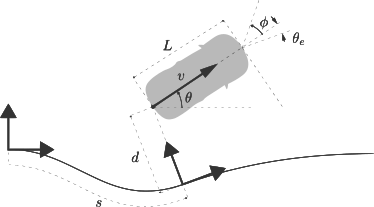
\includegraphics[width=.6\textwidth]{figures/model.pdf}
	\caption{Model of trajectories and the vehicle. Taken from the case study handout.}
	\label{fig:vehicle_model}
\end{figure}
For the dynamic equations several symbols are used. 
Table~\ref{tab:symbols} shows a summary of the symbols used within the document.
\begin{table}[h]
	\centering
	\begin{tabular}{c|l}
	\hline
	\hline
	\textbf{Symbol} & \textbf{Decription}\\
	\hline
		 $s$ & curvilinear coordinate\\
		 $d$ & lateral deviation between vehicle and path\\
		 $\theta_e$ & heading error\\
		 $v$ & longitudinal speed\\
		 $L$ & car length\\
		 $\phi$ & steering wheel angle\\
		 $\alpha$ & speed reference\\
		 $\beta$ & steering wheel angle reference\\
		 $\sigma_a, \sigma_s$ & dynamics of the actuators\\
		 $\kappa(s)$ & curvature of path at position s\\
	\hline
	\hline
	\end{tabular}
	\caption{Symbols used in the dynamics model of the vehicle}
	\label{tab:symbols}
\end{table}

\subsection*{State space model of the Vehicle}
The vehicle is modelled using a set of nonlinear differential equations in state space representation $\mathbf{\dot{x}} = \mathbf{f}(\mathbf{x}, \mathbf{u}, t)$.
The state vector of the system is defined as
\begin{equation}
	\mathbf{x} = \begin{bmatrix}
		x_1, &x_2, &x_3, &x_4, &x_5
	\end{bmatrix} = \begin{bmatrix}
		s, &d, &\theta_e, &v, &\phi
	\end{bmatrix}\, ,
\end{equation}
and the input is
\begin{equation}
	\mathbf{u} = \begin{bmatrix}
		u_1, &u_2	
	\end{bmatrix} = \begin{bmatrix}
		\alpha, &\beta
	\end{bmatrix}\, .
\end{equation}
The model of the vehicle is provided in the case study handout
\begin{eqnarray}
	\dot{x_1} &=& \frac{x_4 \cos(x_3)}{1 - x_2\kappa}\label{eq:ss1}\\
	\dot{x_2} &=& x_4 \sin(x_3)\label{eq:ss2}\\
	\dot{x_3} &=& \frac{x_4}{L}\tan(x_5) - \frac{\kappa x_4 \cos(x_3)}{1 - x_2 \kappa}\label{eq:ss3}\\
	\dot{x_4} &=& \sigma_a (u_1 - x_4)\label{eq:ss4}\\
	\dot{x_5} &=& \sigma_s (u_2 - x_5)\label{eq:ss5}
\end{eqnarray}
For the time being, the state vector is also the output of the model.
